\documentclass[a4paper,11pt,UTF8]{article}
\usepackage{ctex}
\usepackage{amsmath,amsthm,amssymb,amsfonts}
\usepackage{amsmath}
\usepackage[a4paper]{geometry}
\usepackage{graphicx}
\usepackage{microtype}
\usepackage{siunitx}
\usepackage{booktabs}
\usepackage[colorlinks=false, pdfborder={0 0 0}]{hyperref}
\usepackage{cleveref}
\usepackage{esint} 
\usepackage{graphicx}
\usepackage{ragged2e}
\usepackage{pifont}
\usepackage{extarrows}
\usepackage{mathptmx}
\usepackage{float}
\usepackage{caption}
\graphicspath{{./graphics/}} %设置图片路径
% \captionsetup[figure]{name={Figure}}
%opening
\title{运算放大器仿真报告}
\author{董浩\quad 信卓2201 \quad U202213781}
\date{}
\begin{document}
\maketitle
\section{放大电路}
\subsection{同向放大电路}
\begin{figure}[H]
	\centering
	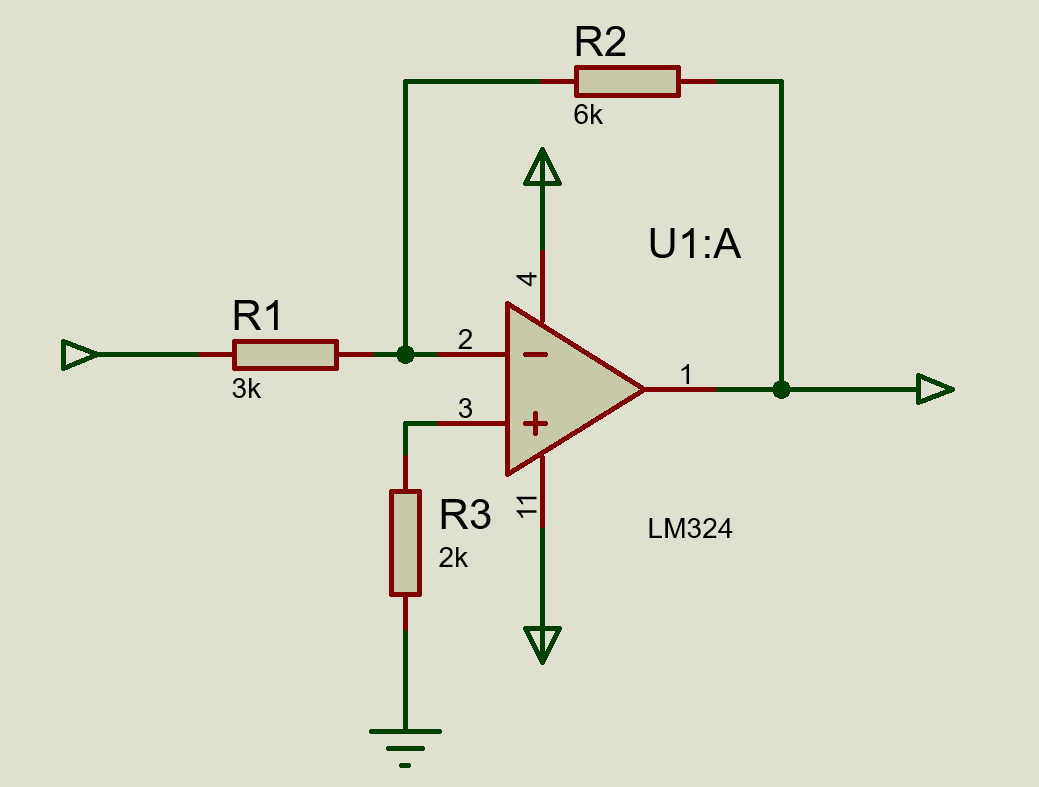
\includegraphics[width=0.5\textwidth]{反向放大器}
	\caption{反向放大器}
\end{figure}
增益:
$$A_v = - \frac{R_2}{R_1}$$

$R_3$的作用为阻抗匹配,取值为$R_1//R_2$.

输入电阻$R_i=R_1$, 输出电阻$R_0 = \infty$.
\subsection{反向放大电路}
\begin{figure}[H]
	\centering
	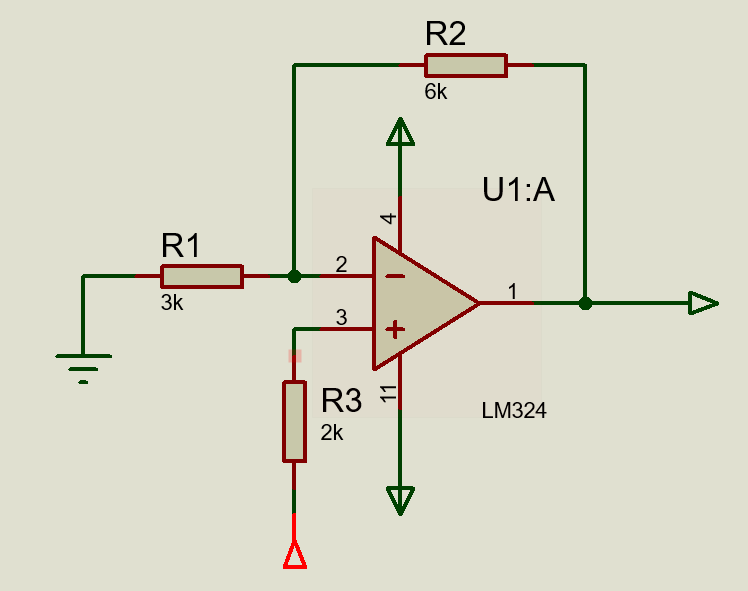
\includegraphics[width=0.5\textwidth]{同向放大器}
	\caption{同向放大器}
\end{figure}
增益:
$$A_v=1+\frac{R_2}{R_1}$$

$R_3$的作用为阻抗匹配,取值为$R_1//R_2$.

输入电阻$R_i=\infty$, 输出电阻$R_0 = \infty$.

\section{加减电路}
\subsection{反向加法器}
\begin{figure}[H]
	\centering
	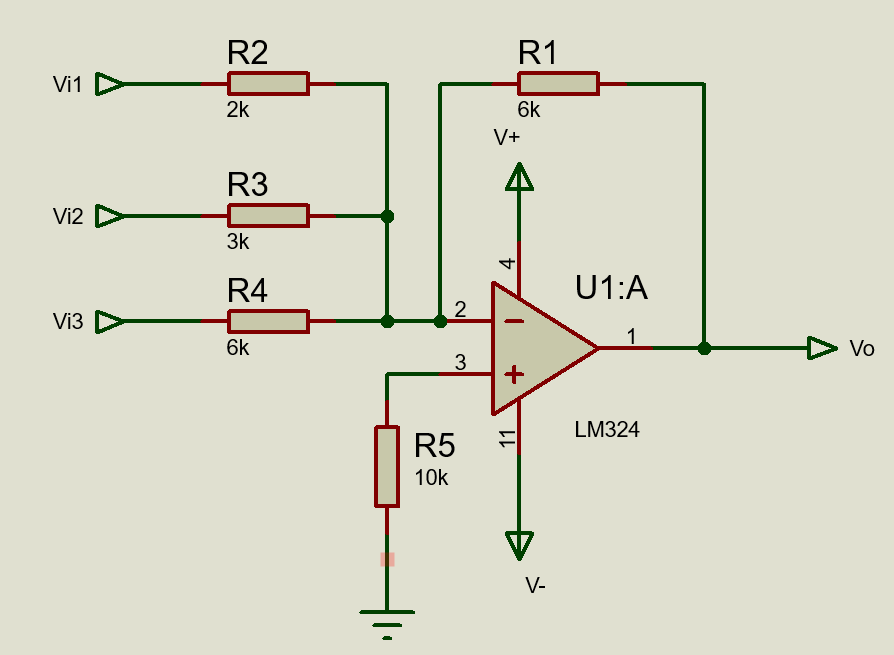
\includegraphics[width=0.5\textwidth]{反向加法器}
	\caption{反向加法器}
\end{figure}
增益:
$$A_v=-(\frac{R_2}{R_1}\cdot V_{i1}+\frac{R_3}{R_1}\cdot V_{i2}+\frac{R_4}{R_1}\cdot V_{i3})$$

$R_5$的作用为阻抗匹配,取值为$R_1//R_2//R_3//R_4$.

根据不同的输入端口,$R_i$取不同的值.

输出电阻:$R_o = \infty$.
\subsection{同向加法器}
\begin{figure}[H]
	\centering
	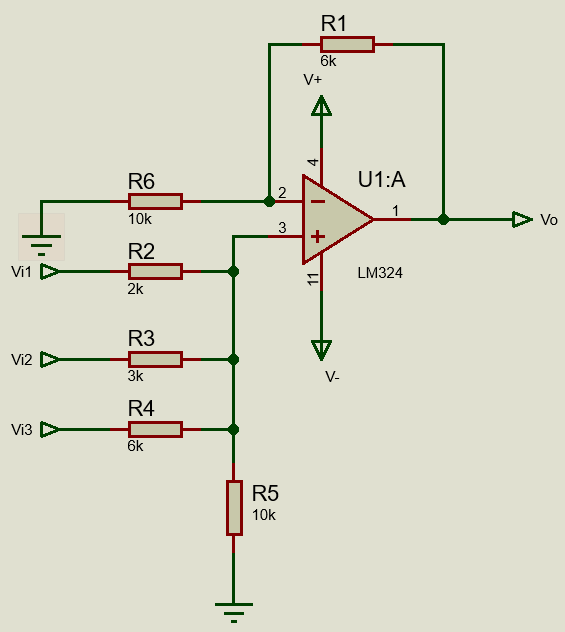
\includegraphics[width=0.5\textwidth]{同向加法器}
	\caption{同向加法器}
\end{figure}
增益:
$$A_v=(1+\frac{R_6}{R_1})\cdot(\frac{R_3//R_4//R_5}{R_2+R_3//R_4//R_5}\cdot V_{i1}+\frac{R_2//R_4//R_5}{R_3+R_2//R_4//R_5}\cdot V_{i2}+\frac{R_2//R_3//R_5}{R_4+R_2//R_3//R_5}\cdot V_{i3})$$

$R_5$的作用为阻抗匹配,可省略,取值满足关系式$R_1//R_6=R_2//R_3//R_4//R_5$.

输入电阻:$R_i=\infty$,输出电阻:$R_o = \infty$.

\subsection{差分减法电路}
\begin{figure}[H]
	\centering
	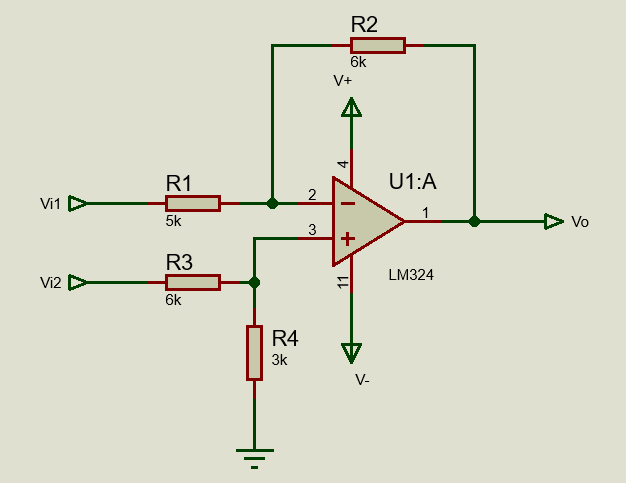
\includegraphics[width=0.5\textwidth]{差分减法电路}
	\caption{差分减法电路}
\end{figure}
传递函数:
$$Vo = (1+\frac{R_2}{R_1})(\frac{\frac{R_4}{R_3}}{1+\frac{R_4}{R_3}})V_{i2}-\frac{R_2}{R_1}V_{i1}$$

特别的,当$\frac{R_4}{R_3}=\frac{R_2}{R_1}$时,有$V_o=\frac{R_2}{R_1}(V_{i2}-V_{i1})$.

根据不同的输入端口,$R_i$取不同的值.

输出电阻$R_o=\infty$.

\section{积分电路}
\subsection{反向积分电路}

\begin{figure}[H]
	\centering
	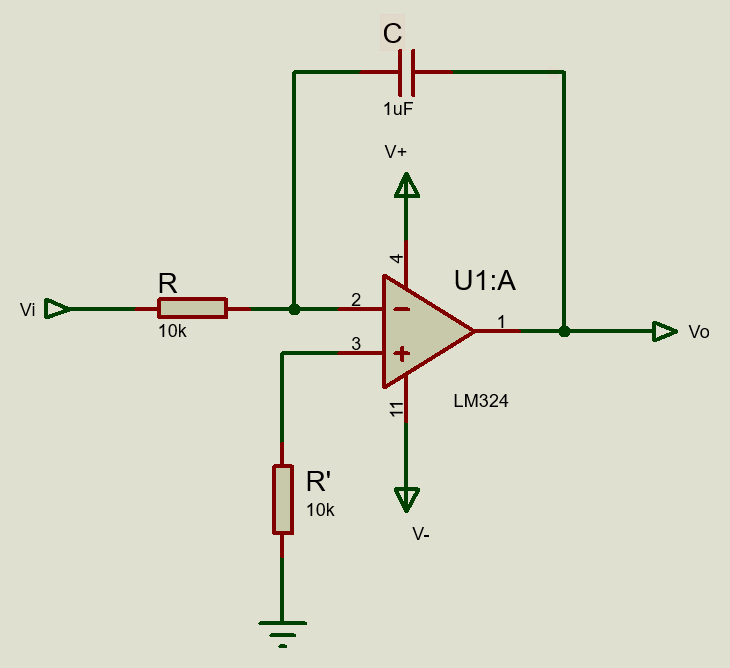
\includegraphics[width=0.5\textwidth]{反向积分电路}
	\caption{反向积分电路}
\end{figure}
传递函数:
$$V_i = -\frac{1}{RC}\int V_i dt$$

输入电阻$R_i=\infty$,输出电阻$R_o=\infty$.

\subsection{实用型反向积分电路}
在使用积分器时,为了防止低频信号增益过高,需在电容旁并联一个电阻加以限制


\begin{figure}[H]
	\centering
	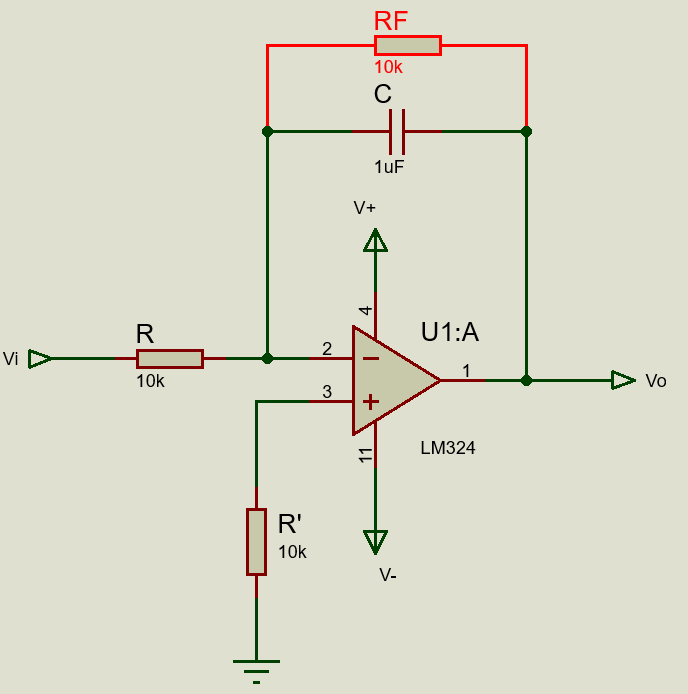
\includegraphics[width=0.5\textwidth]{实用型反向积分电路}
	\caption{实用型反向积分电路}
\end{figure}
电路特性同反向积分电路.

\section{微分电路}
\begin{figure}[H]
	\centering
	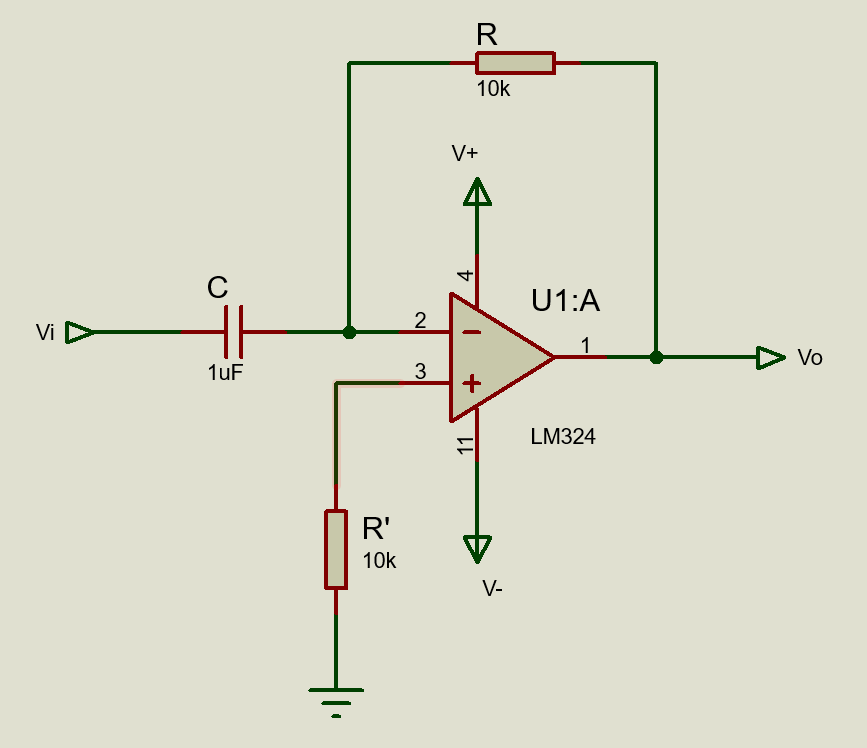
\includegraphics[width=0.5\textwidth]{微分电路}
	\caption{微分电路}
\end{figure}
传输函数:
$$V_o = -RC\frac{dV_i}{dt}$$

输入阻抗:$Z_i=\frac{1}{jwC}$,输出阻抗$Z_o=\infty$.
\section{指数与对数电路}
\subsection{指数运算电路}
\begin{figure}
	\centering
	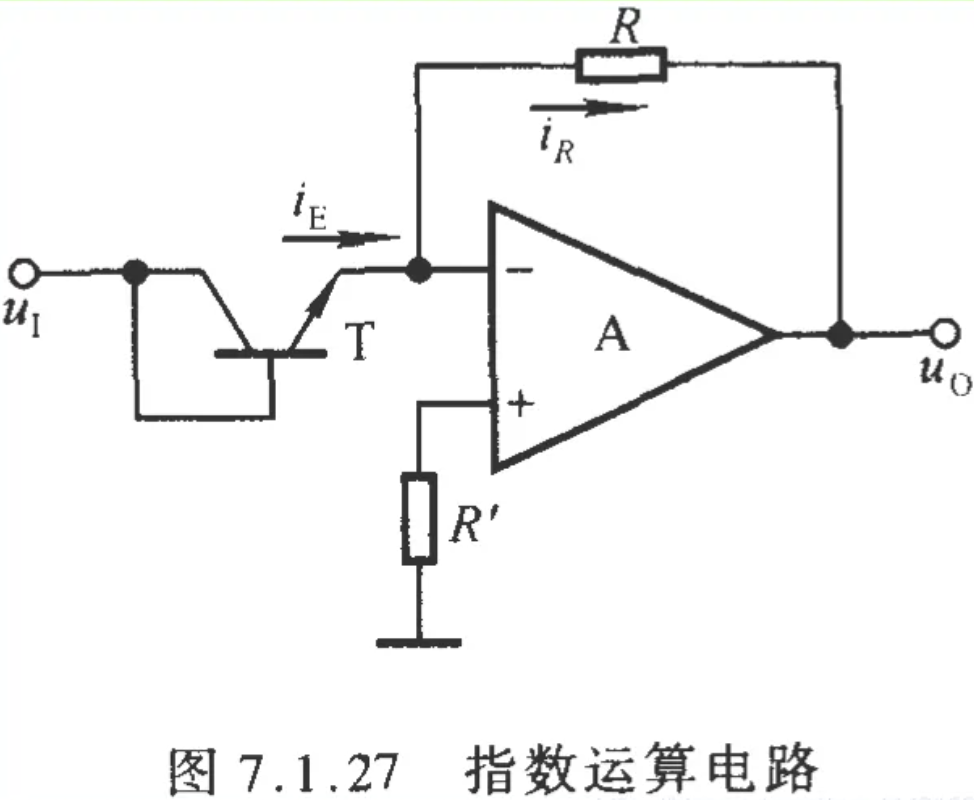
\includegraphics[width=0.5\linewidth]{指数运算电路}
	\caption{指数运算电路}
\end{figure}
\begin{enumerate}
	\item 由于 $u_{N}=0$,则 $u_{BE}=u_{I}$
	\item 由于 $i_{N}=0$,则 $i_{R}=i_{R}=I_{s}e^{ \frac{u_{I}}{U_{T}} }$
	\item 化简,得:
	      $$
		      u_{o}=-i_{R}R=-I_{s}e^{ \frac{u_{I}}{U_{T}}R }
	      $$
\end{enumerate}


\subsection{对数运算电路}
\begin{figure}[H]
	\centering
	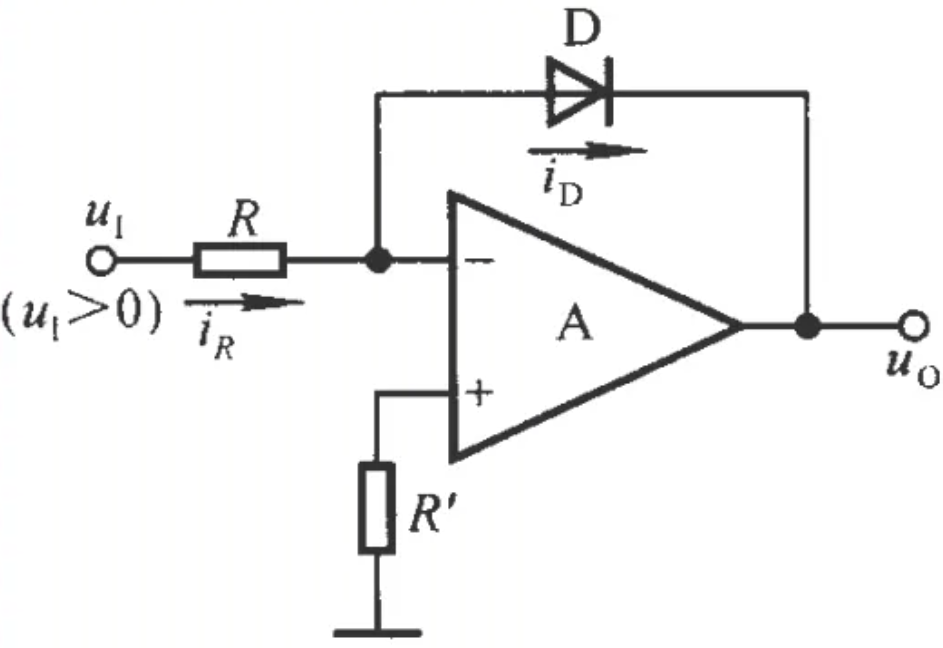
\includegraphics[width=0.5\textwidth]{对数运算电路}
	\caption{对数运算电路}
\end{figure}
\begin{enumerate}
	\item 二极管的正向电流与端电压的关系式:$i_D \approx I_s e^{\frac{u_D}{u_T}}$,故$u_D \approx u_T ln\frac{i_D}{I_s}$
	\item 由于$i_N=0,u_N=0$,则$i_D=i_R=\frac{u_I}{R}$
	\item  由于$u_o=-u_D$化简,得:
	      $$u_o \approx -u_Tln\frac{u_I}{I_sR}$$
\end{enumerate}

%\section{乘除运算电路}


%\section{绝对值运算电路}
\section{滤波器}
\subsection{压控电压源二阶低通滤波器}
\begin{figure}[H]
	\centering
	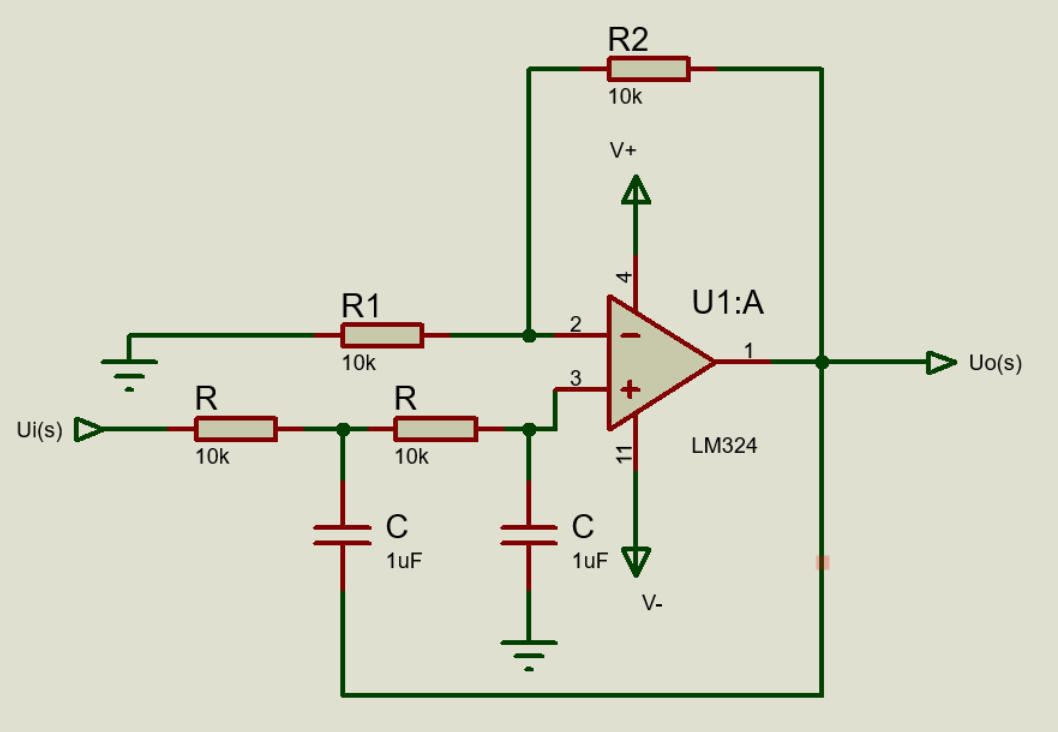
\includegraphics[width=0.5\textwidth]{压控电压源二阶低通滤波器}
	\caption{压控电压源二阶低通滤波器}
\end{figure}
参数选择如下:
$Q = \frac{1}{3-A_{up}}=0.707$;通常放大倍数$A_{up}=1+\frac{R_2}{R_1}$;通带截止频率$f_p$,特征频率$f_o$,$f_p=f_o=\frac{1}{2\pi RC}\\ R_1//R_2=2R$
$$A_u=\frac{U_o(S)}{U_i(S)}=\frac{A_{up}}{1-(\frac{f}{f_{0}})^{2}+j(3+A_{up})\frac{f}{f_{0}}}$$
\subsection{压控电压源二阶高通滤波器}
\begin{figure}[H]
	\centering
	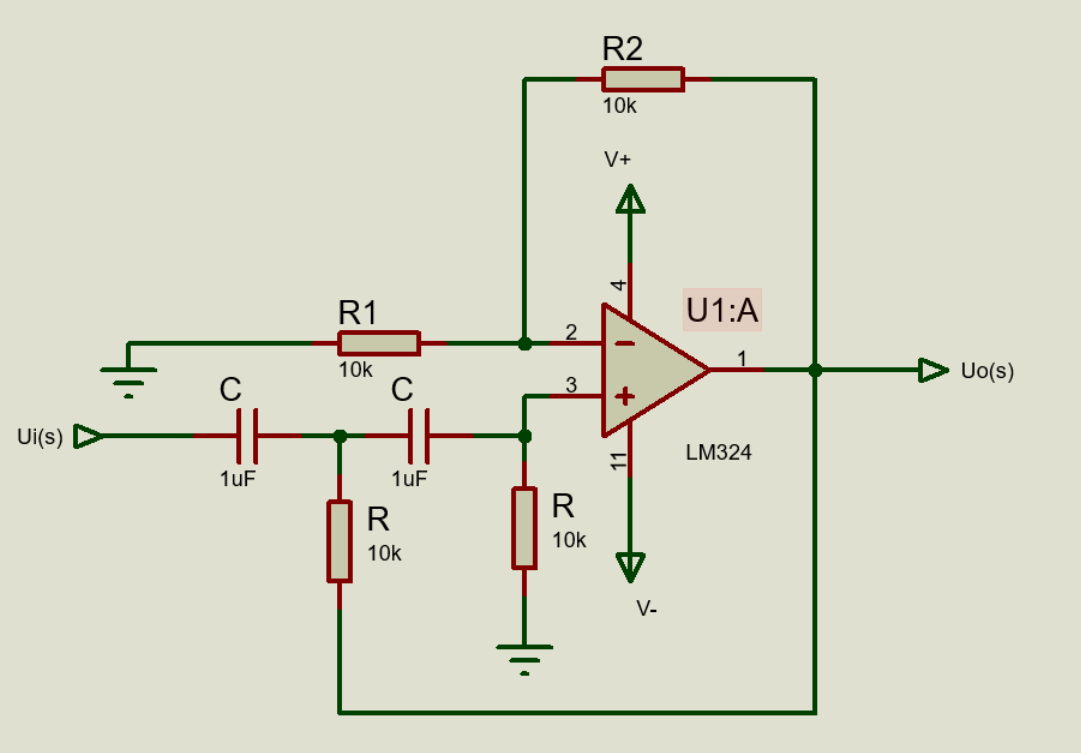
\includegraphics[width=0.5\textwidth]{压控电压源二阶高通滤波器}
	\caption{压控电压源二阶高通滤波器}
\end{figure}
参数选择如下:
$Q=\frac{1}{3-A_{up}}=0.707$;通带放大倍数$A_{up}=1+\frac{R_2}{R_1}$;通带截止频率$f_p$,特征频率$f_o$,$f_p=f_o=\frac{1}{2\pi RC}$, $R_1//R_2=2R$.

$$\left. \begin{array}  { l  }  { A _ { a } = \frac { U _ { o } ( s ) } { U _ { i ( s ) } } } \\ \hspace{1em}{ = \frac { A _ { up } } { 1 - ( \frac { f _ { 0 } } { f } ) ^ { 2 } - 1 + j ( 3 - A _ { up } ) \frac { f _ { 0 } } { f } } } \end{array} \right.$$

\section{信号发生电路}

\subsection{文氏桥震荡电路}
\begin{figure}[H]
	\centering
	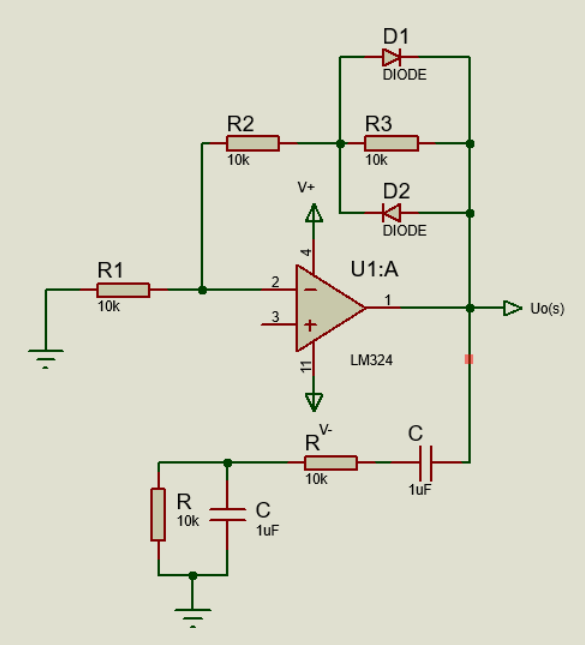
\includegraphics[width=0.5\textwidth]{文氏桥}
	\caption{文氏桥震荡电路}
\end{figure}
震荡频率$f_o = \frac{1}{2\pi RC}$电路起振时应满足$\frac{R_f}{R_1}\geq2$,其中$R_f=R_2+(R_3//R_d)$,$R_d$为二极管正向导通时的等效电阻。$R=R_1//R_f$,D1、D2、$R_3$是起稳幅作用,$R_3$通常选几千欧.
\subsection{方波和三角波发生电路}
\begin{figure}[H]
	\centering
	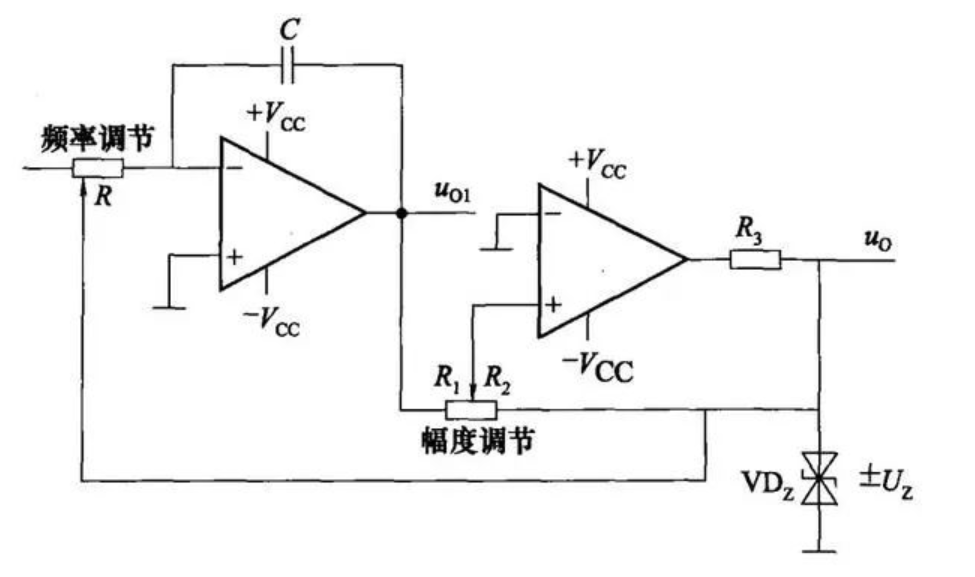
\includegraphics[width=0.5\textwidth]{方波和三角波发生电路}
	\caption{方波和三角波发生电路}
\end{figure}
三角波输出的幅度$U_{O1M}=\pm U_T = \pm \frac{R_1}{R_2}U_z$,方波的幅值$U_{OM}=\pm U_Z$,波形的周期为$T=\frac{4R_1RC}{R_2}$。得到了线性理想的三角波
\subsection{锯齿波发生电路}
\end{document}

